\documentclass[hyperref={pdfpagelabels=false}]{beamer}
\usepackage{lmodern}
\usepackage{graphicx}%este pacote é para figuras
\usepackage[utf8]{inputenc}
\usepackage[brazil]{babel}% este é para o texto
\usepackage[all]{xy}

%\usepackege{multirow,colortbl,array} % estes pacotes são para fazer múltiplas linhas, colorir as celulas e formatar a tabela.

\usepackage{subfig} % este é para fazer sub figuras

\usetheme{Copenhagen}

\title{Mineração de Dados Distribuída Aplicada à Detecção de Desvios Comportamentais no Contexto da Internet das Coisas}  

\author{Ricardo de Azevedo Brand\~{a}o \\ Orientador: Ronaldo Ribeiro Goldschmidt}

\institute {Mestrando em Sistemas e Computação \\ Instituto Militar de Engenharia }

\begin{document}
\begin{frame}
\titlepage
\end{frame} 

\begin{frame}
	\frametitle{Tópicos abordados}
	\footnotesize{\tableofcontents}
\end{frame} 

\section{Introdução}

\subsection{Contextualiza\c{c}\~{a}o}

\begin{frame}
	\frametitle{Introdução}
	\begin{figure}[h]
		\centering
		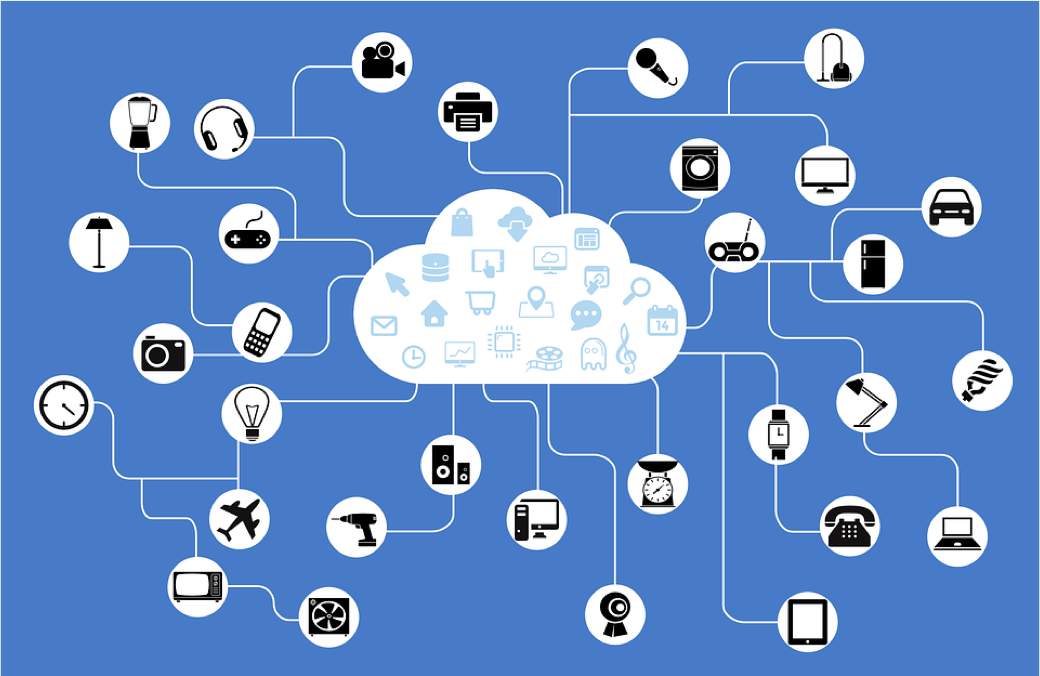
\includegraphics[scale=0.45]{img/IoT.png}
		\caption{\scriptsize{Internet das coisas (Fonte: Creative Commons).}}
		\label{fig:IoT}
	\end{figure}	

\end{frame}

\begin{frame}
	\frametitle{Motivação}

	\begin{itemize}
    	\item Internet das coisas 
	        \begin{itemize}
    	    	\item Coisas (sensores e atuadores) conectadas
       		   	\item Internet (Identificadas por IP)
          		\item Dados Gerados
                	\begin{itemize}
                    	\item Sobre as coisas
                        \item Interação Humanos x Humanos
                        \item Interação Humanos x Coisas
                        \item Interação Coisas x Coisas
                    \end{itemize}
        	\end{itemize}
	\end{itemize}		
\end{frame}

\begin{frame}
	\frametitle{Motivação}
    
	\begin{itemize}
		\item Crescimento expondencial de coisas conectadas
		    \begin{figure}
 		   		\centering
	        	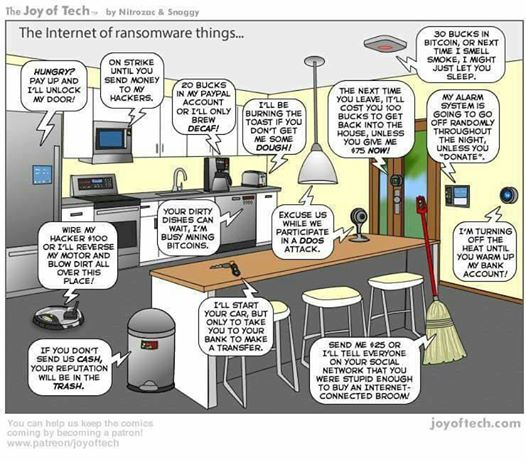
\includegraphics[scale=0.3]{img/ransomwareIoT.jpeg}
  		    	\caption{\scriptsize{Fonte: Joy of Tech http://www.geekculture.com/joyoftech/joyarchives/2340.html}}
   			\end{figure}
	\end{itemize}   
\end{frame}

\subsection{Problema}
 
\begin{frame}

	\frametitle{Problema}	

	\begin{itemize}
    	\item Desafios \cite{000-000} \begin{itemize}
        	\item Centralização na análise de dados \begin{itemize}
      	    	\item Aumento no tráfego da rede
			\end{itemize}
       		\item Topologia Dinâmica \begin{itemize}
          		\item Nós aparecem e desaparecem
               	\item Mudanças constantes no tempo e espaço
			\end{itemize}
        \end{itemize}
        \item Coleta de dados sobre interações \begin{itemize}
        	\item Identificação de desvios de comportamentos de Humanos e Coisas
        	\end{itemize}
	\end{itemize}
    
\end{frame}
 
\subsection{Hipótese}
 
\begin{frame}
	\frametitle{Hipótese}
	
    \begin{itemize}
    	\item O uso de t\'{e}cnicas de minera\c{c}\~{a}o de dados distrubu\'{i}da no cenário da Internet das Coisas pode contribuir para reduzir o tráfego de informações necessárias na análise de padrões de comportamento sem diminuir a qualidade do trabalho se comparado com a identificação de padrões utilizando técnicas de mineração de dados centralizada.
    \end{itemize}
\end{frame}

\subsection{Objetivo}
 
\begin{frame}
	\frametitle{Objetivo}

	\begin{itemize}
		\item Demonstrar que o uso de t\'{e}cnicas de minera\c{c}\~{a}o de dados distrubu\'{i}da no cenário da Internet das Coisas pode contribuir para reduzir o tráfego de informações necessárias na análise de padrões de comportamento sem diminuir a qualidade do trabalho se comparado com a identificação de padrões utilizando técnicas de mineração de dados centralizada. 
	\end{itemize}

\end{frame}

\subsection{Método}  

\begin{frame}
	\frametitle{Método}
     \begin{itemize}
        	\item Revisão da Literatura
            \item Aprofundamento dos conceitos básicos
            \item Escolha de técnicas para implementação
            \item Análise e escolha dos estudos de caso
            \item Preparação dos datasets
            \item Implementação dos algoritmos
            \item Realização dos experimentos
		\end{itemize}

\end{frame}
    
\subsection{Contribuições Esperadas}  

\begin{frame}
	\frametitle{Contribuições Esperadas}

\end{frame}
   

\section{Conceitos Básicos}

\begin{frame}
	\frametitle{Conceitos Básicos}
    
    \Large{Internet Das Coisas} \\
    
    \normalsize{De acordo com \cite{000-004}} é a tecnologia que permitiu a mudança da Internet que conecta dispositivos de usuários finais para uma Internet usada para interconectar objetos físicos que se comunicam entre si e/ou com seres humanos para prover um determinado serviço.
    \begin{itemize}
	    \item \normalsize{Conceito construído em três pilares:} \begin{itemize}
		    \item Deve ser identificável
            \item Deve comunicar-se
            \item Deve Interagir
		    \end{itemize}
        
    \end{itemize}

\end{frame}

\section {Trabalhos relacionados}

\begin{frame}
	\frametitle{Trabalhos relacionados}
    
    Em \cite{000-000} é apresentado um survey sobre Mineração de dados para Internet das Coisas. \\
    Apresenta os desafios agrupados por:
	\begin{itemize}
		\item Infraestrutura
        \item Dados
        \item Algoritmos
        \item Segurança/Privacidade
	\end{itemize}

\end{frame}

\section{Solução Proposta}

\begin{frame}
	\frametitle{Recordando o objetivo do trabalho}
   
   	\begin{center}
	   	\xymatrix{A\ar[r]&B}
   	\end{center}
   
    \begin{figure}[h]
    	\centering
	    
\includegraphics[scale=0.6]{img/drawing.eps}
        \caption{Ret\^{a}ngulo}
    \end{figure}

\end{frame}

\subsection{Visão Geral}  

\begin{frame}
	\frametitle{Visão Geral}
   
\end{frame}
       
\subsection{Viabilidade}  

\begin{frame}
	\frametitle{Viabilidade}
   
\end{frame}

\section{Plano de Ação}

\subsection{Atividades}

\subsection{Cronograma}
\begin{frame}
	\frametitle{Cronograma}
\end{frame}


\section {Referências}
\begin{frame}
\frametitle{Bibliografia}
    \bibliographystyle{apalike}
    \small{ \bibliography{ref} }
\end{frame}

\end{document}

